
\newcommand{\linenumber}[1]{\texttt{\textcolor{gray}{#1\ }}}
\newcommand{\textgray}[1]{\texttt{\textcolor{gray}{#1}}}

\newcommand{\texttug}[1]{\texttt{\textcolor{tug}{#1}}}
\newcommand{\texttugbo}[1]{\textbf{\texttt{\textcolor{tug}{#1}}}}
\newcommand{\texttugb}[1]{\texttt{\textcolor{tugb!120}{#1}}}
\newcommand{\textblack}[1]{\texttt{#1}}
\newcommand{\textblackb}[1]{\textbf{\texttt{#1}}}
\newcommand{\textorang}[1]{\texttt{\textcolor{color4}{#1}}}
\newcommand{\textgreen}[1]{\texttt{\textcolor{tugb!120}{#1}}}

\begin{tikzpicture}[node distance=1mm, font=\tiny, line width=0.15pt]

    \node [shape=rectangle,fill=none, inner sep=0pt, align=center] (dataset) {
      \fontsize{4.5}{4.5}\selectfont
      \setlength\arrayrulewidth{0.2pt}
      \addtolength{\tabcolsep}{-0.9em}
      \renewcommand{\arraystretch}{1.3}
      \hspace{-4pt}
      \begin{tabular}{|c@{\hskip 0.1em}|c@{\hskip 0.1em}|c@{\hskip 0.1em}|c@{\hskip 0.1em}|c@{\hskip 0.1em}|} 
          \hline
          \multicolumn{5}{|c@{\hskip 0.1em}|}{\cellcolor{lightgray!10}\texttt{Salary dataset: comma-separated CSV file}} \\
          \multicolumn{5}{|c@{\hskip 0.1em}|}{\cellcolor{lightgray!10}\texttt{Target feature: "\textbf{Salary}"}}
           \\ \hline  
          \rowcolor{tugb!10}
          \textbf{\texttt{Experience}}& \textbf{\texttt{Skills}}& \textbf{\texttt{Gender}}& \textbf{\texttt{Address}}& \textbf{\texttt{Salary}}\\ \hline    
          \texttt{12 Months} &  \texttt{SQL,Java} & \texttt{F} & \texttt{7050 CA} & \texttt{100} \\ \chline
          \rowcolor{lightgray!20}
          \texttt{two years} &  \texttt{JavaScript} & \texttt{Female} & \texttt{TX 7871} & \texttt{150} \\ \chline
          \texttt{36 months} &  \texttt{C/C++,.Net} & \texttt{M} & \texttt{Texas} & \texttt{300} \\ \chline
          \rowcolor{lightgray!20}
          \texttt{3 Years} &  \texttt{JS,CPP,SQL} & \texttt{Female} & \texttt{7871} & \texttt{310} \\ \chline
          \texttt{one Year} &  \texttt{Python} & \texttt{Male} & \texttt{CA} & \texttt{200} \\ \chline
          \rowcolor{lightgray!20}
          \texttt{2 Years} &  \texttt{C\#,Java} & \texttt{0} & \texttt{TX} & \texttt{175} \\ %\chline
          %\texttt{...} &  \texttt{...} & \texttt{...} & \texttt{...} & \texttt{...} \\ 
          \hline                    
        \end{tabular}
    };  
  
%    \node[right=of dataset, inner sep=0, xshift=-2pt, yshift=-26pt] (catdbpip){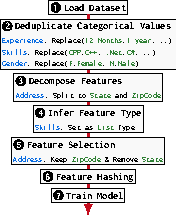
\includegraphics[scale=0.9]{img/fig_catdb_pipDAG.pdf}}; 
   \node[below=of dataset, inner sep=0, xshift=10pt, yshift=-8pt] (metadatapip) {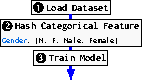
\includegraphics[scale=0.9]{img/fig_metadata_pipDAG.pdf}}; 
   
%    \draw[-{Latex[scale=0.7]},line width=0.8pt, tug] ($(dataset.north east)+(-1.2pt,-10pt)$) -- ($(dataset.north east)+(22pt,-10pt)$);
   \draw[line width=0.8pt, blue] ($(dataset.south)+(10pt,0pt)$) -- (metadatapip);

%    \node[below=of catdbpip, inner sep=0pt, yshift=2pt] {Accuracy = 91.8\%};
   \node[below=of metadatapip, inner sep=0pt, yshift=2pt] {Accuracy = 39.2\%};

%    \node[inner sep=0, above=of catdbpip, text=tug] {\textbf{\tiny{\texttt{Pipeline DAG with CatDB \& LLM}}}};
   \node[inner sep=0, above=of metadatapip, rotate=0, yshift=-3pt, xshift=-35pt, text=blue] {
    \shortstack[l]{\textbf{\tiny{\texttt{Pipeline DAG with}}} \vspace{-2pt}\\
    \textbf{\tiny{\texttt{Metadata \& LLM}}}}
    };
    
\end{tikzpicture}
